% This file was created by tikzplotlib v0.9.5.
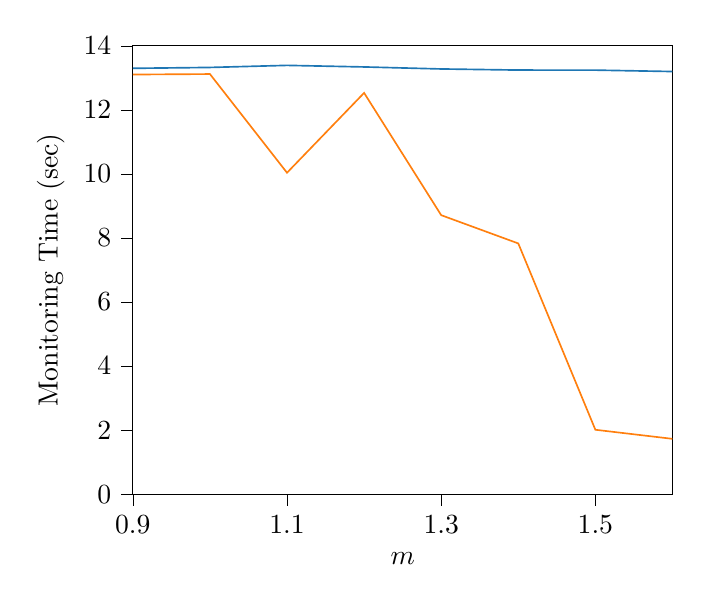
\begin{tikzpicture}

\definecolor{color0}{rgb}{0.12156862745098,0.466666666666667,0.705882352941177}
\definecolor{color1}{rgb}{1,0.498039215686275,0.0549019607843137}

\begin{axis}[
tick align=outside,
tick pos=left,
x grid style={white!69.0196078431373!black},
xlabel={\(\displaystyle m\)},
xmin=0, xmax=7,
xtick style={color=black},
xtick={-0,2,4,6,8},
xticklabels={0.9,1.1,1.3,1.5,1.7},
y grid style={white!69.0196078431373!black},
ylabel={Monitoring Time (sec)},
ymin=0, ymax=14,
ytick style={color=black},
ytick={-0,2,4,6,8,10,12,14},
yticklabels={\(\displaystyle {0}\),\(\displaystyle {2}\),\(\displaystyle {4}\),\(\displaystyle {6}\),\(\displaystyle {8}\),\(\displaystyle {10}\),\(\displaystyle {12}\),\(\displaystyle {14}\)}
]
\addplot [semithick, color0]
table {%
0 13.2969665227036
1 13.3244687355997
2 13.3890030500959
3 13.3400586041986
4 13.2769666102031
5 13.2424736907007
6 13.2403752513041
7 13.1967877566
};
\addplot [semithick, color1]
table {%
0 13.1030873316005
1 13.1181511283983
2 10.036142073902
3 12.5295692500978
4 8.7111693724044
5 7.82862510219711
6 2.0100999243994
7 1.72649138319684
};
\end{axis}

\end{tikzpicture}
